 \documentclass[pdftex,12pt, oneside]{article}

%\usepackage[paperwidth=8.5in, paperheight=13in]{geometry} % Folio
\usepackage[paperwidth=8.27in, paperheight=11.69in]{geometry} % A4

\usepackage{makeidx}         % allows index generation
\usepackage{graphicx}        % standard LaTeX graphics tool
                             % when including figure files
\usepackage[bottom]{footmisc}% places footnotes at page bottom
\usepackage[english]{babel}
\usepackage{enumerate}
\usepackage{paralist}
\usepackage{float}
\usepackage{gensymb}  
\usepackage{listings}
\usepackage{color}
\usepackage{mathtools} % atau \usepackage{amsmath}
\renewcommand{\baselinestretch}{1.5}

\newcommand{\HRule}{\rule{\linewidth}{0.5mm}}

\definecolor{codegreen}{rgb}{0,0.6,0}
\definecolor{codegray}{rgb}{0.5,0.5,0.5}
\definecolor{codepurple}{rgb}{0.58,0,0.82}
\definecolor{backcolor}{rgb}{0.95,0.95,0.92}

\lstdefinestyle{mystyle}{
  backgroundcolor=\color{backcolor},
  commentstyle=\color{codegreen},
  keywordstyle=\color{magenta},
  stringstyle=\color{codepurple},
  basicstyle=\footnotesize,
  breakatwhitespace=false,
  breaklines=true,
  captionpos=b,
  keepspaces=true,
  numbers=left,
  numbersep=5pt,
  showspaces=false,
  showstringspaces=false,
  showtabs=false,
  tabsize=2
}

\lstset{style=mystyle}


\begin{document}
\sloppy % biar section ga melebar melewati kertas

\begin{center}
{\large RANCANGAN SISTEM BASIS DATA - WS PBB}
\\[1cm]
XX Februari 2017\\
Priyanto Tamami, S.Kom.
\end{center}

%\frontmatter%%%%%%%%%%%%%%%%%%%%%%%%%%%%%%%%%%%%%%%%%%%%%%%%%%%%%%


%%%%%%%%%%%%%%%%%%%%%%%%%%%%%%%%%%%%%%%%%%%%%%%%%%%%%%%%%%%%%%%%%%%%%%

\section{PENDAHULUAN}

Aplikasi \textit{Web Services} ini bertujuan untuk melakukan pencatatan pembayaran pada basis data SISMIOP yang dilakukan oleh Bank sebagai tempat pembayaran.

Aplikasi ini sesungguhnya tidak menggunakan basis data baru, melainkan menggunakan basis data yang sudah ada, yaitu basis data yang digunakan pada SISMIOP, dimana tabel yang terpengaruh atas pencatatan pembayaran ada dua, yaitu tabel SPPT, dan tabel PEMBAYARAN\_SPPT.

Agar setiap transaksi yang terjadi dapat dievaluasi penggunaannya, maka diperlukan tabel tambahan yang mencatat \textit{log} transaksi, baik pencatatan pembayaran, atau pembatalan pencatatan pembayaran (\textit{reversal}).


\section{STRUKTUR BASIS DATA}

Struktur basis data dapat digambarkan sebagai berikut :

\subsection{Struktur Tabel SPPT}

Tabel ini sebetulnya sudah terbentuk dan dimanfaatkan oleh aplikasi SISMIOP untuk menampung data tagihan Pajak Bumi dan Bangunan Perdesaan dan Perkotaan yang dihasilkan setiap tahun. Tabel ini akan digunakan dalam aplikasi \textit{Web Service} PBB sebagai data dasar penentuan jumlah pembayaran yang akan dikirimkan atas permintaan \textit{inquiry} dari Bank sebagai tempat pembayaran.

Strukturnya adalah seperti pada gambar \ref{fig:tabel-sppt} :

\begin{figure}[H]
  \centering
  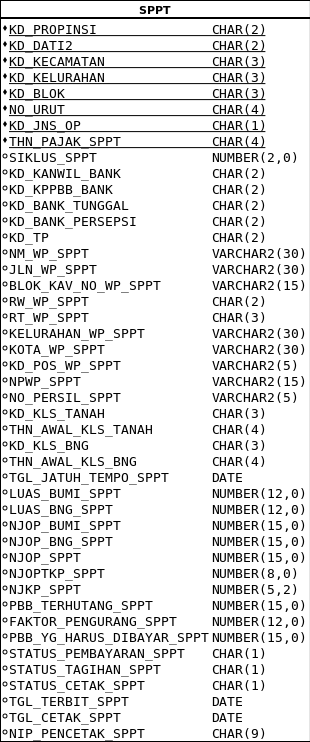
\includegraphics[width=0.4\textwidth]{./resources/01-struktur-tabel-sppt}
  \caption{Struktur Tabel SPPT}
  \label{fig:tabel-sppt}
\end{figure}

\subsection{Struktur Tabel PEMBAYARAN\_SPPT}

Tabel ini pun sudah terbentuk dan dimanfaatkan oleh aplikasi SISMIOP untuk mencatat transaksi pembayaran secara manual oleh operator. Tabel ini digunakan pula pada aplikasi \textit{Web Service} PBB untuk mencatat pembayaran yang terjadi.

Struktur dari tabel PEMBAYARAN\_SPPT ini adalah seperti pada gambar \ref{fig:tabel-pembayaran-sppt} :

\begin{figure}[H]
  \centering
  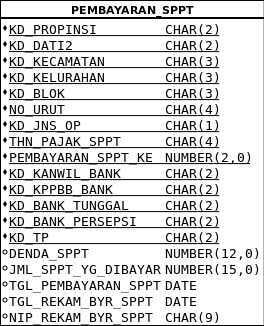
\includegraphics[width=0.4\textwidth]{./resources/02-struktur-tabel-pembayaran-sppt}
  \caption{Struktur Tabel PEMBAYARAN\_SPPT}
  \label{fig:tabel-pembayaran-sppt}
\end{figure}

\subsection{Struktur Tabel DAT\_OP\_BUMI}

Tabel ini sudah terbentuk dan dimanfaatkan oleh aplikasi SISMIOP untuk menampung data bumi dan objek pajak bumi dan bangunan. Tabel ini akan terisi pada saat operator memasukkan data-data pada lembar Surat Pemberitahuan Objek Pajak (SPOP). 

Struktur dari tabel DAT\_OP\_BUMI ini seperti pada gambar \ref{fig:tabel-dat-op-bumi} : 

\begin{figure}[H]
	\centering
	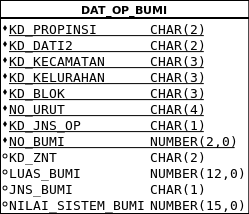
\includegraphics[width=0.4\textwidth]{./resources/03-struktur-tabel-dat-op-bumi}
	\caption{Struktur Tabel DAT\_OP\_BUMI}
	\label{fig:tabel-dat-op-bumi}
\end{figure}

\subsection{Struktur Tabel REF\_KELURAHAN}

Tabel ini sudah terbentuk dan dimanfaatkan oleh aplikasi SISMIOP untuk menampung data administrasi Desa/Kelurahan seperti nama Desa/Kelurahan, kode pos, dan sebagainya. Tabel ini digunakan pada aplikasi \textit{Web Service} PBB untuk melakukan \textit{inquiry} terhadap nama Desa/Kelurahan.

Struktur dari tabel REF\_KELURAHAN ini adalah seperti pada gambar \ref{fig:tabel-ref-kelurahan} :

\begin{figure}[H]
  \centering
  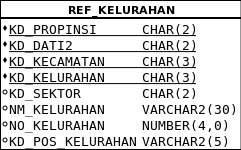
\includegraphics[width=0.4\textwidth]{./resources/04-struktur-tabel-ref-kelurahan}
  \caption{Struktur Tabel REF\_KELURAHAN}
  \label{fig:tabel-ref-kelurahan}
\end{figure}

\subsection{Struktur Tabel REF\_KECAMATAN}

Tabel ini sudah terbentuk dan dimanfaatkan oleh aplikasi SISMIOP untuk menampung data administrasi Kecamatan. Tabel ini digunakan pada aplikasi \textit{Web Service} PBB untuk memberikan informasi nama Kecamatan pada proses \textit{inquiry} dan pencatatan pembayaran PBB-P2.

Struktur dari tabel REF\_KECAMATAN ini adalah seperti pada gambar \ref{fig:tabel-ref-kecamatan} :

\begin{figure}[H]
	\centering
	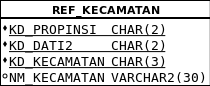
\includegraphics[width=0.4\textwidth]{./resources/05-struktur-tabel-ref-kecamatan}
	\caption{Struktur Tabel REF\_KECAMATAN}
	\label{fig:tabel-ref-kecamatan}
\end{figure}

\subsection{Struktur Tabel LOG\_TRX\_PEMBAYARAN}

Tabel ini adalah tabel baru yang digunakan untuk menyimpan catatan terhadap proses transaksi pembayaran melalui aplikasi \textit{Web Service} PBB.

Struktur dari tabel LOG\_TRX\_PEMBAYARAN ini adalah seperti pada gambar \ref{fig:tabel-log-trx-pembayaran} :

\begin{figure}[H]
  \centering
  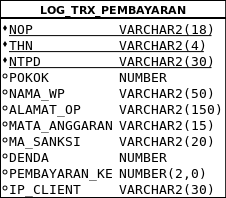
\includegraphics[width=0.4\textwidth]{./resources/06-struktur-tabel-log-trx-pembayaran}
  \caption{Struktur Tabel LOG\_TRX\_PEMBAYARAN}
  \label{fig:tabel-log-trx-pembayaran}
\end{figure}

Yang menjadi \textit{field} atau data penting pada tabel ini adalah NOP, Tahun Pajak (THN), dan Nomor Transaksi Pajak Daerah (NTPD). \textit{Field} inilah yang nantinya menjadi kunci dari setiap transaksi yang terjadi pada sistem aplikasi \textit{Web Service} PBB.


\subsection{Struktur Tabel LOG\_REVERSAL}

Tabel ini digunakan sebagai tempat untuk menyimpan catatan tarhadap proses \textit{reversal} atau koreksi data pembayaran yang telah terjadi sebelumnya.

Struktur dari tabel LOG\_REVERSAL ini adalah seperti pada gambar \ref{fig:tabel-log-reversal} :

\begin{figure}[H]
	\centering
	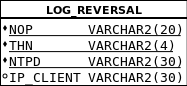
\includegraphics[width=0.4\textwidth]{./resources/07-struktur-tabel-log-reversal}
	\caption{Struktur Tabel LOG\_REVERSAL}
	\label{fig:tabel-log-reversal}
\end{figure}


\section{DIAGRAM RELASI \textit{ENTITY}}

Diagram relasi yang menggambarkan hubungan antar tabel pada sistem aplikasi \textit{Web Service} PBB adalah seperti pada gambar \ref{fig:relasi-entity} :

\begin{figure}[H]
	\centering
	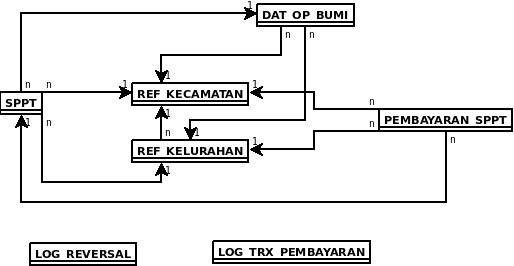
\includegraphics[width=0.8\textwidth]{./resources/08-relasi-entity}
	\caption{Diagram Relasi}
	\label{fig:relasi-entity}
\end{figure}

Yang dapat dijabarkan sebagai berikut, tabel SPPT akan bergantung dengan data yang berada pada tabel DAT\_OP\_BUMI, dimana satu data pada tabel DAT\_OP\_BUMI akan ada banyak data di tabel SPPT, karena setiap Nomor Objek Pajak pada tabel DAT\_OP\_BUMI akan ditetapkan pada tabel SPPT setiap tahun pajak.

Tabel SPPT pun akan bergantung dengan data pada tabel REF\_KECAMATAN dan REF\_KELURAHAN, dimana satu Kecamatan dan satu Desa/Kelurahan akan memiliki banyak objek di tabel SPPT. 



\end{document}